\documentclass[a4paper]{article}

% --------------------------------------------------
% Encoding (wichtig für pdfLaTeX)
% --------------------------------------------------
\usepackage[utf8]{inputenc}
\usepackage[T1]{fontenc}

% --------------------------------------------------
% Schrift (Alternative zu Mulish)
% --------------------------------------------------
\usepackage{tgheros} % modern, clean sans-serif
\renewcommand{\familydefault}{\sfdefault}

% --------------------------------------------------
% Mathematics & Science
% --------------------------------------------------
\usepackage{amsmath,amssymb,mathtools,bm}
\usepackage{siunitx}
\usepackage[version=4]{mhchem}
\usepackage{chemformula}
\usepackage{bigints}
\usepackage[official]{eurosym}

\numberwithin{equation}{subsection}

% --------------------------------------------------
% Graphics & Figures
% --------------------------------------------------
\usepackage{graphicx}
\usepackage{float}
\usepackage{subfigure}
\usepackage{subcaption}
\usepackage{caption}
\captionsetup[subfigure]{justification=centering}
\usepackage[justification=centering]{caption}
\usepackage{sidecap}

% --------------------------------------------------
% Tables
% --------------------------------------------------
\usepackage{booktabs}
\usepackage{tabularx}
\usepackage{longtable}

% --------------------------------------------------
% Lists & Code
% --------------------------------------------------
\usepackage{enumitem}
\usepackage{listings}

% --------------------------------------------------
% Misc
% --------------------------------------------------
\usepackage{subfiles}
\usepackage{pdfpages}
\usepackage{comment}
\usepackage{textgreek}
\usepackage{cite}

% --------------------------------------------------
% Colors
% --------------------------------------------------
\usepackage{xcolor}

\definecolor{TUred}{RGB}{196,30,58}

% --------------------------------------------------
% Hyperlinks
% --------------------------------------------------
\usepackage[
    colorlinks=true,
    linkcolor=black,
    citecolor=TUred,
    urlcolor=TUred
]{hyperref}

% --------------------------------------------------
% Layout
% --------------------------------------------------
\usepackage[rmargin=2cm,lmargin=2cm,tmargin=2.5cm]{geometry}

\setlength{\parindent}{0pt}
\setlength{\parskip}{1ex plus 0.5ex minus 0.2ex}

% --------------------------------------------------
% Section formatting
% --------------------------------------------------
\usepackage{titlesec}

\titleformat{\section}
{\Large\bfseries\color{TUred}}
{\thesection}
{1em}
{}

\titleformat{\subsection}
{\large\bfseries\color{TUred}}
{\thesubsection}
{1em}
{}

\titleformat{\subsubsection}
{\normalsize\bfseries\color{TUred}}
{\thesubsubsection}
{1em}
{}

% --------------------------------------------------
% TikZ
% --------------------------------------------------
\usepackage{tikz}
\usetikzlibrary{shapes.geometric,arrows}

\tikzstyle{startstop} = [rectangle, rounded corners, minimum width=3cm, minimum height=1cm, text centered, draw=black, fill=gray!20]
\tikzstyle{process}   = [rectangle, minimum width=3cm, minimum height=1cm, text centered, draw=black, fill=blue!10]
\tikzstyle{decision}  = [diamond, minimum width=3cm, minimum height=1cm, text centered, draw=black, fill=red!10]
\tikzstyle{arrow}     = [thick,->,>=stealth]

% --------------------------------------------------
% Units
% --------------------------------------------------
\DeclareSIUnit{\wattpeak}{Wp}

% --------------------------------------------------
% Header / Footer
% --------------------------------------------------
\usepackage{fancyhdr}

\pagestyle{fancy}
\fancyhf{}

\fancyhead[C]{\color{TUred}Energy Systems -- Group Project}
\fancyfoot[C]{\color{TUred}Summer Semester 2026}

\renewcommand{\headrulewidth}{0pt}
\renewcommand{\footrulewidth}{0pt}

% --------------------------------------------------
% Boxes
% --------------------------------------------------
\usepackage{tcolorbox}
\tcbuselibrary{skins,breakable}

\newtcolorbox{notebox}{
    colback=gray!10!white,
    colframe=gray!80!black,
    title=Note,
    breakable
}

\newtcolorbox{commentbox}{
    colback=red!5!white,
    colframe=TUred,
    title=Comment,
    breakable
}

\newtcolorbox{cautionbox}{
    colback=yellow!5!white,
    colframe=yellow!75!black,
    title=Caution,
    breakable
}

% --------------------------------------------------
% Document
% --------------------------------------------------
\begin{document}

\begin{titlepage}
    \centering
    \vspace*{\stretch{0.1}}
    
    \vspace{2cm}
    
    \fontsize{18}{24}\selectfont  % Increased line spacing from 20 to 24
    \Huge \textbf{\textcolor{TUred}{Energy Systems - Group Project}}
    
    \vspace{1.5cm}  % Increased from 1cm
    
    \large
    Group O\\
    
    \vspace{0.5cm}  % Added spacing before names
    
    \begin{tabular}{ll}
    Valentin Barranco Martinez & ()\\
    Ole Hangen & (456334)\\
    Spiridon Giacco Phil Jaeger-Gatidis & ()\\
    Tobias Alexander Knauf & (386265)\\
    Niklas Teitge & (403240)\\
    \end{tabular}
    
    \vspace*{\stretch{1}}
    
    \normalsize
    \begin{flushleft}
        \normalsize Department of Digital Transformation in the Energy Sector\\
        Technical University Berlin\\
        \today
    \end{flushleft}
    
    \hfill
    
\includegraphics[width=5cm]{Images/TuBerlin_Logo.png}
\end{titlepage}

\newpage
\setcounter{page}{1}

\section{Task 1 - Questions on primal solution}

\textbf{
    (a) Compute the annuity factor a(r,L) and the annualised costs for the technologies. \\
    Output: Table (0.5)
    }

With $r=7\%$ and the following equations for the annuity factor $a(r,L)$ and the annualised costs $c_{inv}$ 

\begin{equation*}
    a(r,L) = \frac{r(1+r)^L}{(1+r)^L - 1}
\end{equation*}

\begin{equation*}
    c_{\mathrm{inv}}
    = \mathrm{overnight} \cdot a(r,L)
    + \mathrm{FOM}
\end{equation*}

we receive these values for the different technologies:

\begin{table}[ht]
    \centering
    \small
    \setlength{\tabcolsep}{4pt}
    \begin{tabularx}{\textwidth}{l l r r r r r r r}
        \toprule
        Component   & Kind  & $c_{\mathrm{var,other}}$  & Overnight Cost   & FOM    & Lifetime    & Efficiency  & Annuity Factor & $c_{\mathrm{inv}}$ \\
        \midrule
        Wind                & power            & 1.62 & 1,286,467 & 15,148 & 30     & --   & 0.08 & 118,819.75  \\
        Solar               & power            & 0.00 & 367,867   & 9,304  & 40     & --   & 0.08 & 36,897.39   \\
        H2 electrolyser     & charge power     & 0.00 & 1,257,335 & 50,293 & 25     & 0.70 & 0.09 & 158,185.57  \\
        H2 fuel cell        & discharge power  & 0.00 & 1,068,642 & 53,432 & 10     & 0.50 & 0.14 & 205,582.58  \\
        H2 storage          & energy           & 0.00 & 1,604     & 0      & 100    & --   & 0.07 & 112.41      \\
        Battery inverter    & power            & 0.00 & 80,223    & 722    & 10     & 0.96 & 0.14 & 12,143.95   \\
        Battery storage     & energy           & 0.00 & 100,279   & 0      & 30     & --   & 0.08 & 8,081.12    \\
        Line                & power            & 0.00 & 1,544,274 & 23,164 & 40     & --   & 0.08 & 138,998.66  \\
        \bottomrule
    \end{tabularx}
    \caption{Annuity factor and annualised costs for the technologies}
    \label{tab:tech_parameters}
\end{table}

\textbf{
    (b) In the no-line case, what does the dispatch of solar and wind look like in each node? \\
    Output: Dispatch plot (0.5)
    }

To find the optimal solution in the no-line case we minimize the objective function subject to the constraints and receive with the dual-simplex algorithm the value of

\begin{equation*}
    \min z = 3\,412\,846\,097.4\,\text{€}
\end{equation*}

The optimal dispatch results for the no-line case for solar and wind in each node are shown in \autoref{fig:1b_dispatch solar and wind - no line case}. A second output in \autoref{fig:1b_storage dispatch} illustrates how storage systems participate in the dispatch pattern.

\begin{figure}[!htbp]
    \centering
    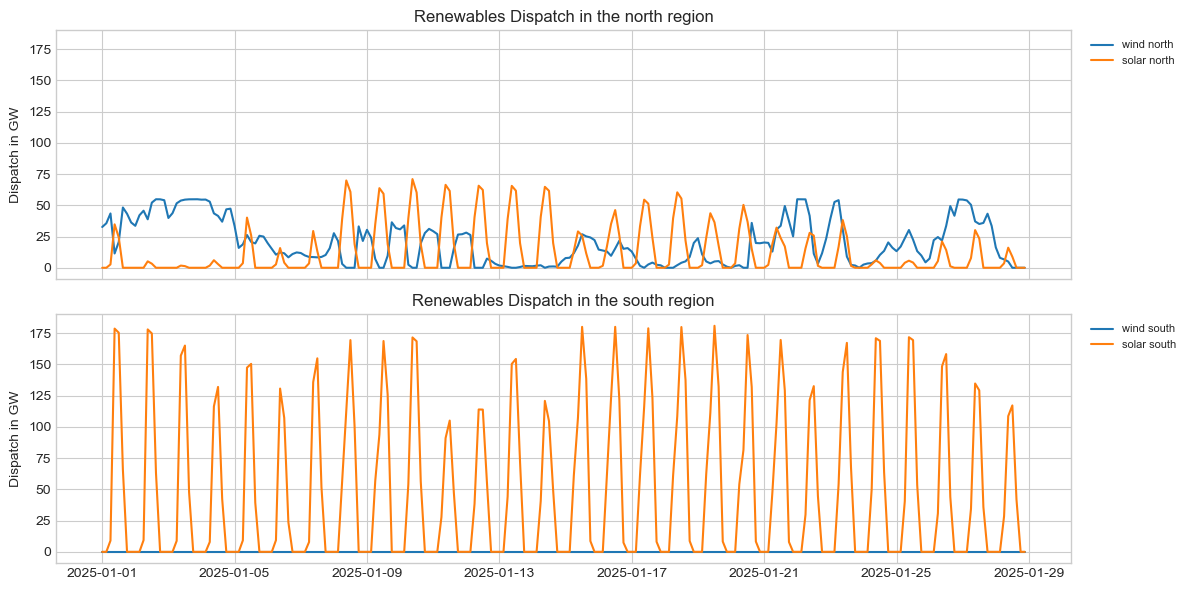
\includegraphics[width=1\linewidth]{Images/1b_wind_solar_dispatch.png}
    \caption{Dispatch of solar and wind in each node in the no-line case}
    \label{fig:1b_dispatch solar and wind - no line case}
\end{figure}

\begin{figure}[!htbp]
    \centering
    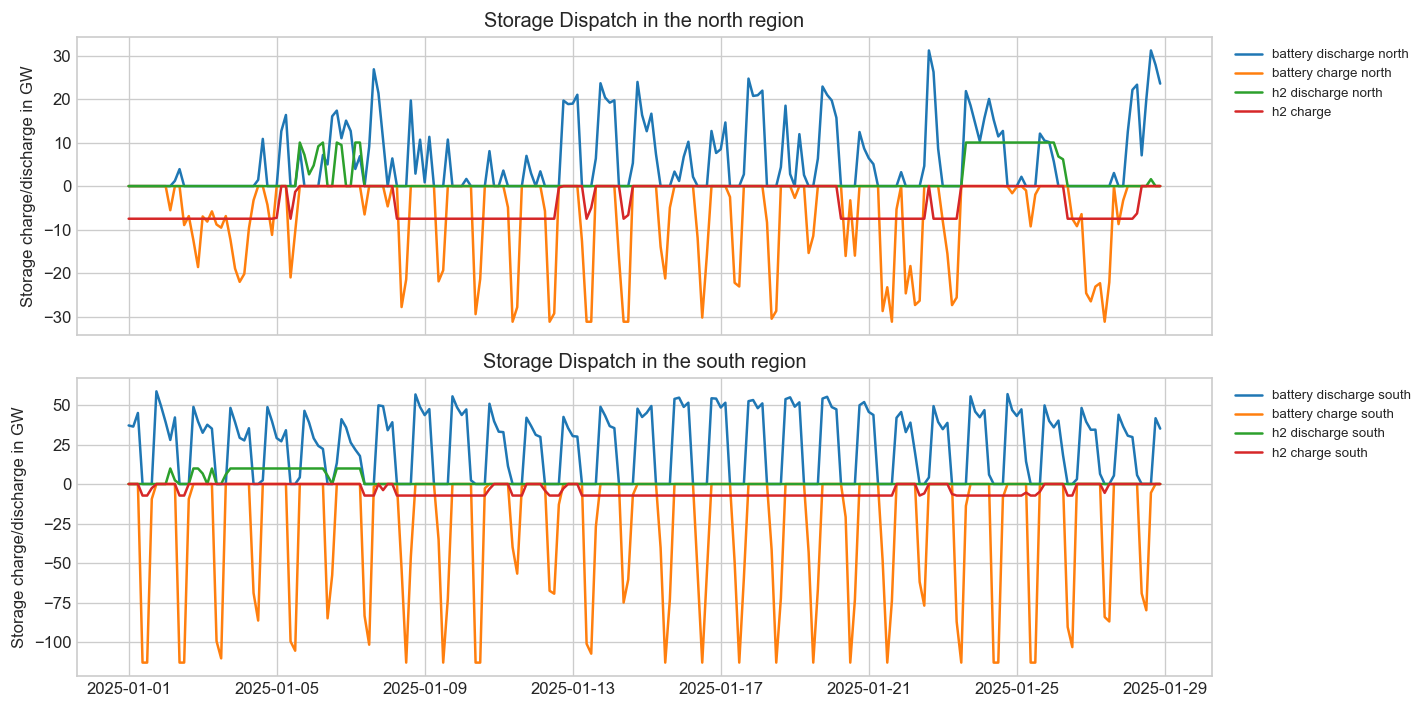
\includegraphics[width=1\linewidth]{Images/1b_storage dispatch.png}
    \caption{Participation of storage systems in the dispatch pattern in each node}
    \label{fig:1b_storage dispatch}
\end{figure}

It can be observed that wind and solar are combined only in the northern node, whereas the southern node instead uses a combination of solar power and storage. This is due to several reasons. In scenario B (no line) each node has to cover its own demand, so the dispatch follows the local resource. \\
Generation dispatch: \\
In the north the supply is a mix of wind and solar. Wind carries the base supply across day and night and dominates in winter, while solar adds generation during the daytime hours, so the dispatch stays relatively
continuous. In the south no wind is built at all, so solar is the only source. Its dispatch is strongly diurnal: high peaks around midday and zero at night, with large swings between the seasons. \\
Storage dispatch: \\
Because the north already has a fairly balanced wind-solar mix, it needs less storage. The south depends entirely on solar, which produces nothing at night, so a lot of energy has to be shifted from day to night.
That is why both the battery and the H2 charge/discharge power and storage capacity are clearly higher in the south. Batteries handle the short day-night cycle, while H2 covers the longer, seasonal shifts.
Overall this split is the solver's least-cost choice: it follows the local production potential (north = windiest node, south = sunniest node) together with the technology costs.

\textbf{
    (c) Compare the two scenarios. How do the investments into generation, storage, and transmission change? \\
    Output: Show the investment costs in a table and plot the capacities.(1)
    }

The following \autoref{tab:1c_optimal_solution} shows the optimal solution for scenarios A and B, as well as savings through line inclusion (which is the cost of B - A) and the build line capacity in scenario A. 

\begin{table}[h]
    \centering
    \begin{tabular}{l r}
        \hline
        TOTEX Scenario A (line) & 3\,056\,740\,408.5\,\text{€}      \\
        TOTEX Scenario B (no line) & 3\,412\,846\,097.4\,\text{€}   \\
        Savings through line inclusion & 356\,105\,688.9\,\text{€}  \\
        Build line capacity & 14.06 GW                              \\
        \hline
    \end{tabular}
    \caption{Optimal solution for scenarios A and B – investment cost and build line capacity}
    \label{tab:1c_optimal_solution}
\end{table}

Furthermore, \autoref{tab:1c_annual_costs_comparison_every_tech} compares the annual costs of each technology across both scenarios. The third column in the table indicates whether a technology is more expensive in the line or no-line case. Positive values indicate higher annual costs in scenario A (line), whereas negative values indicate higher annual costs in scenario B (no line). 
%A visualization of the table is given in \autoref{fig:1c_inv_costs_tech_A_vs_B}.

\begin{table}[ht]
    \centering
    \begin{tabular}{l r r r}
        \hline
        Component & A (line) [Mio€/a] & B (no line) [Mio€/a] & $\Delta$ A--B [Mio€/a] \\
        \hline
        Wind                & 8\,385  & 6\,858  & 1\,527    \\
        Solar               & 15\,714 & 19\,105 & -3\,391   \\
        H2 electrolyser     & 859     & 2\,343  & -1\,484   \\
        H2 fuel cell        & 1\,824  & 4\,078  & -2\,254   \\
        H2 storage          & 167     & 359     & -192      \\
        Battery inverter    & 1\,536  & 1\,751  & -215      \\
        Battery storage     & 9\,085  & 9\,714  & -629      \\
        Line                & 1\,954  & 0       & 1\,954    \\
        \hline
    \end{tabular}
    \caption{Annual costs comparison between scenarios A and B for every technology}
    \label{tab:1c_annual_costs_comparison_every_tech}
\end{table}

%\begin{figure}
%    \centering
%    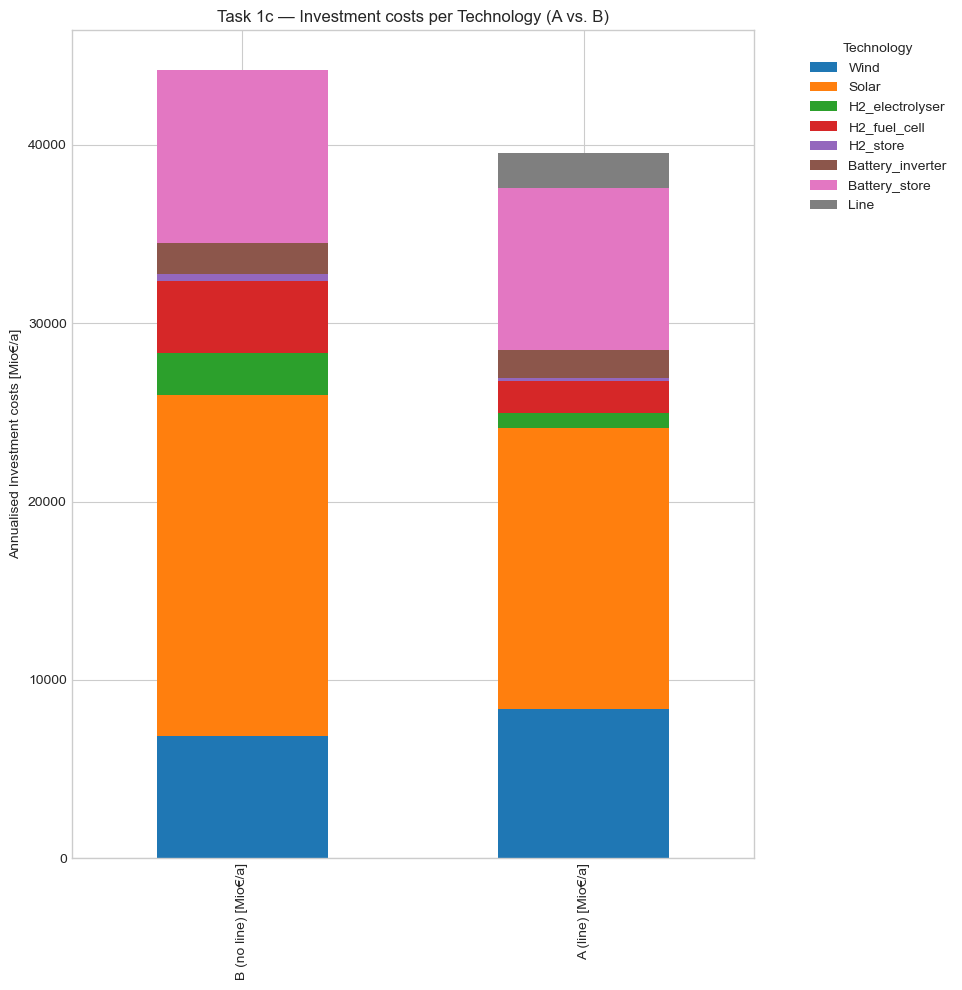
\includegraphics[width=0.7\linewidth]{Images/1c_inv_costs_tech_A_vs_B.png}
%    \caption{Investment costs of the different technologies in scenarios A (line) and B (no line)}
%    \label{fig:1c_inv_costs_tech_A_vs_B}
%\end{figure}

\autoref{fig:1c_powercap_vs_energycap} shows the comparison of the power and energy capacity in each node and for either scenarios. 

\begin{figure}[!htbp]
    \centering
    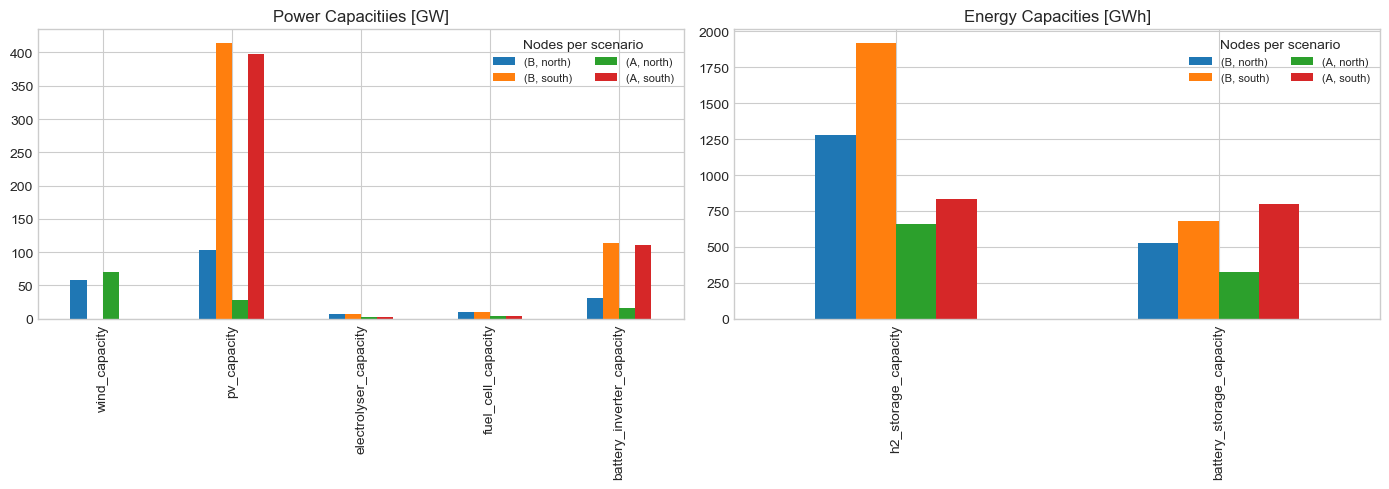
\includegraphics[width=1\linewidth]{Images/1c_power_cap_vs_energy_cap.png}
    \caption{Power and energy capacity for each node and scenario}
    \label{fig:1c_powercap_vs_energycap}
\end{figure}

The total investment costs shrink when line capacity is built (TOTEX falls from ~3.41 to ~3.06 billion €). With the line the regions no longer have to cover their demand on their own, so they can specialise. \\
Generation: \\
The north expands wind and strongly cuts its solar, turning into a cheap wind exporter, while the south stays solar-based. Wind in the north is favourable because its good resource potential combined with the costs helps to reduce total costs. The south keeps its strong solar potential and only needs to reduce its storage and a little of its production capacity to meet demand. \\
Storage: \\
Because excess energy can be transferred between regions instead of being stored locally, less storage is needed overall. This is mostly visible in the H2 storage (it drops by roughly half) and in the northern battery, while the southern battery even grows slightly. \\
Transmission: \\
Line capacity is built to carry the energy and to smooth the supply across seasonal and day/night differences between the windy north and the sunny south.

\textbf{
    (d) How does curtailment by technology and region change from the no-line case to the transmission case and why? \\
    Output: Quantify and explain. (0.5)
    }

The curtailment of wind and solar generation in the respective regions is shown in Figures \ref{fig:1d_curtailment_time_series} and \ref{fig:1d_curtailment_quantified}. \autoref{fig:1d_curtailment_time_series} illustrates the curtailment over time for each scenario, while \autoref{fig:1d_curtailment_quantified} presents the corresponding values aggregated over time and disaggregated by technology and node. \autoref{tab:1d_curtailment_quantified} provides the numerical values underlying the visualization in \autoref{fig:1d_curtailment_quantified}.

\begin{figure}[!htbp]
    \centering
    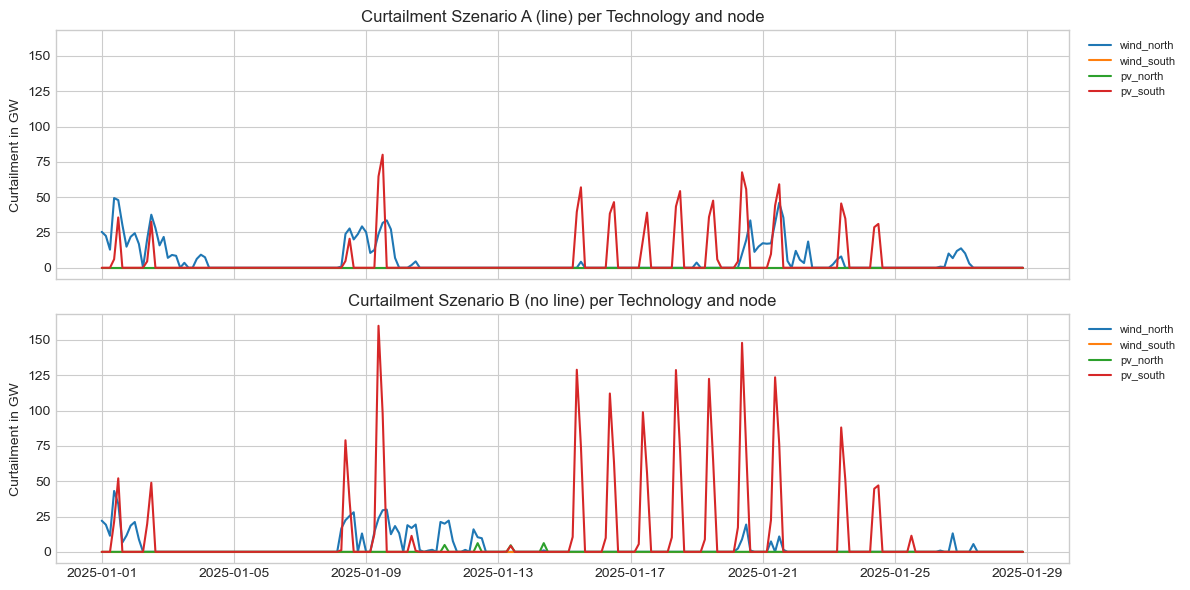
\includegraphics[width=1\linewidth]{Images/1d_curtailment_time_series.png}
    \caption{Times series of curtailment in each scenario}
    \label{fig:1d_curtailment_time_series}
\end{figure}

\begin{figure}[!htbp]
    \centering
    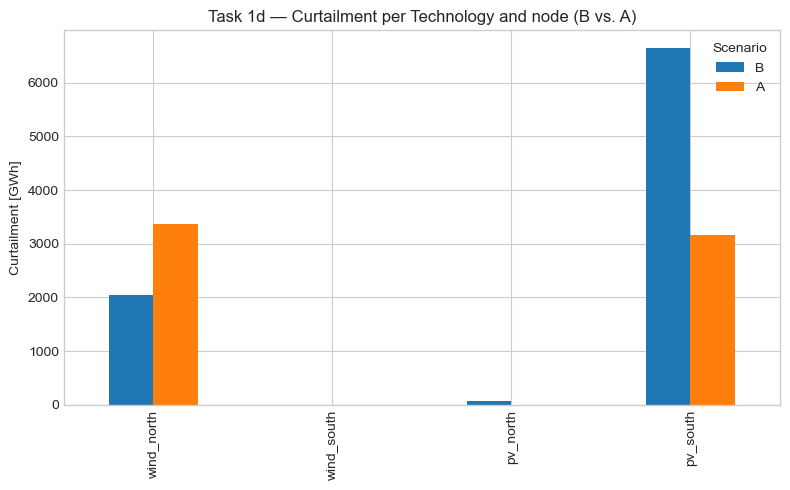
\includegraphics[width=1\linewidth]{Images/1d_curtailment_qunatified.png}
    \caption{Curtailment in GWh for each technology, region and scenario}
    \label{fig:1d_curtailment_quantified}
\end{figure}

\begin{table}[!htbp]
    \centering
    \begin{tabular}{l r r}
        \hline
        Technology and Region & Scenario A [GWh] & Scenario B [GWh] \\
        \hline
        Wind north   & 2\,044 & 3\,376  \\
        Wind south   & 0      & 0       \\
        Solar north  & 66     & 0       \\
        Solar south  & 6\,641 & 3\,169  \\
        \hline
    \end{tabular}
    \caption{Curtailment in GWh for each technology, region and scenario}
    \label{tab:1d_curtailment_quantified}
\end{table}

Total curtailment falls when the line is built, but it does not fall everywhere. \\
South PV:   \\ Curtailment drops strongly. In the no-line case the south has a large midday solar surplus that it cannot use or store, so it has to be spilled. With the line this surplus can be exported to the north instead of being curtailed. \\
North wind: \\ Curtailment actually increases. With the line the north overbuilds cheap wind to export it. During high-wind hours the line and storage cannot always absorb all of it, so a larger share of the wind potential is spilled.\\
North PV:   \\ Drops to zero because the north barely builds any solar anymore in the line scenario. So the line reduces overall curtailment by letting the regions share their surplus, but it shifts the remaining curtailment towards the technology that is deliberately overbuilt for export (northern wind).

\textbf{
    (e) How do the residual load curves change across the two scenarios? \\
    Output: Plot the residual load curves and explain the differences. (0.5)
    }

\autoref{fig:1e_residual_load} illustrates the residual load curve for the line and no-line cases.

The residual load is defined as the difference between electricity demand and dispatched renewable generation, aggregated over both nodes and sorted into a duration curve:
\begin{equation*}
    R(t) = D(t) - G_{\text{RES}}(t)
\end{equation*}

where $R(t)$ denotes the residual load, $D(t)$ the total demand, and $G_{\text{RES}}(t)$ the dispatched renewable generation.

Positive values of $R(t)$ represent residual demand that must be covered by storage, while negative values indicate surplus renewable generation that is absorbed by storage.

\begin{figure}[!htbp]
    \centering
    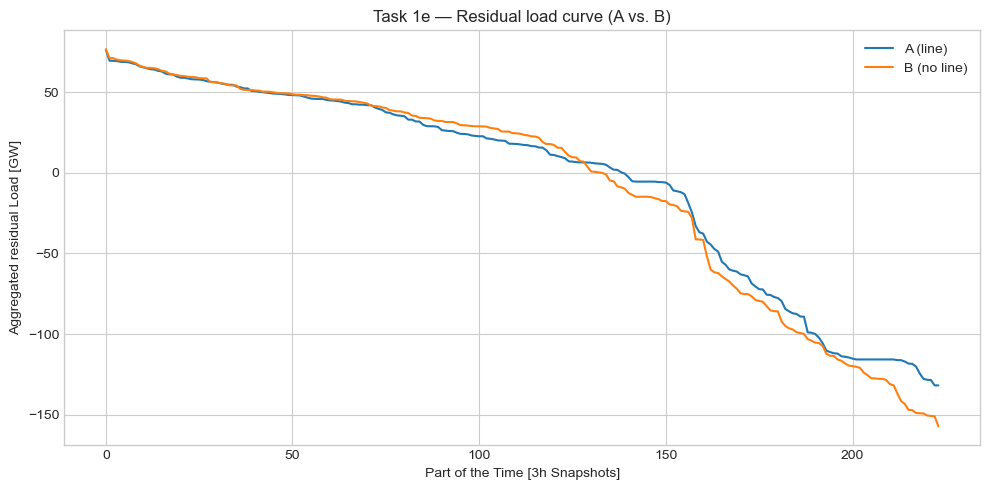
\includegraphics[width=1\linewidth]{Images/1e_residual_load.png}
    \caption{Residual load curve of scenarios A and B}
    \label{fig:1e_residual_load}
\end{figure}

The peak of the curve is almost identical in both scenarios. This corresponds to the system-wide situation in which neither wind nor PV generation is available. When both regions simultaneously experience low wind and solar availability, the transmission line cannot provide additional support, since no surplus energy is available for spatial balancing. Consequently, storage must cover the demand. The main difference appears at the negative (surplus) end of the curve: with the transmission line, the curve is significantly flatter. The line enables spatial balancing of non-simultaneous surpluses between regions (northern wind and southern solar), thereby reducing the amount of energy that needs to be shifted through storage. This is consistent with the results in Sections 1c and 1d: with transmission, the system relies less on storage (resulting in lower hydrogen capacities) and experiences less curtailment, as spatial exchange partially substitutes temporal storage.
\newpage
\section{Task 2 - Questions on dual solution}

\textbf{(a) For each scenario, extract the shadow variable to the nodal energy balances and weight it by the nodal demand in the north and south, respectively. What do they represent? Why are they different in the two regions? When do you observe the highest values and why? (0.5)}

\textbf{(b) In the transmission scenario, consumers of which region benefit more from the transmission line: the north, the south, or both equally? Briefly explain. (0.5)}

\textbf{(c) Extract the shadow price of the line capacity constraint in the transmission scenario. What does it represent? In the scenario where the transmission capacity is zero, you can also extract the dual variable. Comparing the two, what does it say about the value of interconnection? (0.5)}

\textbf{(d) Which advantages and disadvantages of heavy reliance on cross-regional interconnection does this stylised model not capture? No calculation needed. (0.5)}

%\newpage
%\addcontentsline{toc}{section}{References}
%\bibliographystyle{unsrt}
%\bibliography{Bibliography}

%\newpage
%\appendix
%\input{Appendix}

\end{document}